\documentclass{article}

% 导入中文宏包
\usepackage{array}
\usepackage{caption}
\usepackage{ctex}
\usepackage{hyperref}
% 设置页面边距
\usepackage{geometry}
\usepackage{graphicx}
\geometry{a4paper, left=2cm, right=2cm, top=3cm, bottom=4cm}

% 设置标题、作者和日期
\title{Shell工具与Vim编辑器的学习}
\author{23020007073  刘畅}

\begin{document}

% 生成标题、作者和日期
\maketitle

% 心得报告正文
\section{实验目的}
本次课程主要了解了Shell工具,脚本,编辑器Vim以及数据整理。

\section{练习内容}
\subsection{Shell学习样例10个}

1.echo "Hello, World!"用Shell打印hello world
echo 是一个在命令行界面(shell)中常用的命令,它能够输出一段文本或者变量的值到标准输出

\noindent
\begin{minipage}{\linewidth}
  \centering
  % 插入图片
  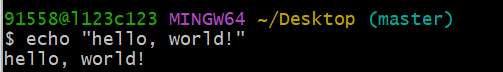
\includegraphics[width=0.5\linewidth]{echo.png}
  % 图片标题
  \captionof{figure}{echo 用来显示文本或变量}
  \label{fig:example}
\end{minipage}


2.变量赋值及调用

\noindent
\begin{minipage}{\linewidth}
  \centering
  % 插入图片
  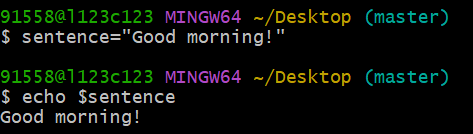
\includegraphics[width=0.5\linewidth]{fuzhi.png}
  % 图片标题
  \captionof{figure}{变量的赋值和使用}
  \label{fig:example}
\end{minipage}

3.加法运算

\noindent
\begin{minipage}{\linewidth}
	\centering
	% 插入图片
	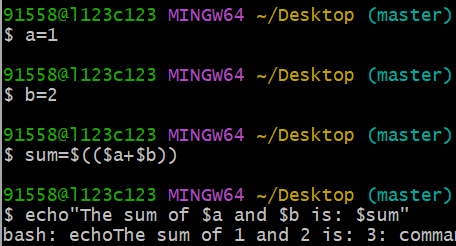
\includegraphics[width=0.5\linewidth]{sum.png}
	% 图片标题
	\captionof{figure}{进行加法运算}
	\label{fig:example}
\end{minipage}

4.条件语句的判断

\noindent
\begin{minipage}{\linewidth}
  \centering
  % 插入图片
  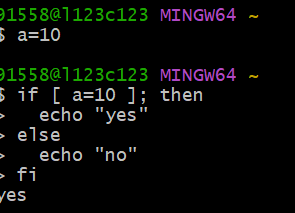
\includegraphics[width=0.5\linewidth]{if.png}
  % 图片标题
  \captionof{figure}{条件语句的判断}
  \label{fig:example}
\end{minipage}

5.循环的使用

\noindent
\begin{minipage}{\linewidth}
 \centering
  % 插入图片
  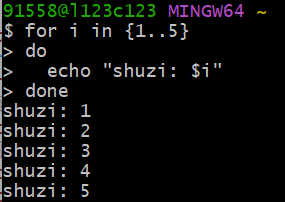
\includegraphics[width=0.5\linewidth]{for.png}
  % 图片标题
  \captionof{figure}{循环语句}
  \label{fig:example}
\end{minipage}

6.函数的创建和使用

\noindent
\begin{minipage}{\linewidth}
	\centering
	% 插入图片
	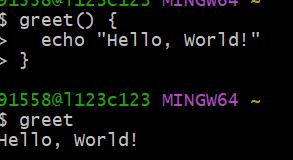
\includegraphics[width=0.5\linewidth]{greet.png}
	% 图片标题
	\captionof{figure}{定义函数与使用}
	\label{fig:example}
\end{minipage}

7.文件的创立与写入

\noindent
\begin{minipage}{\linewidth}
 \centering
  % 插入图片
  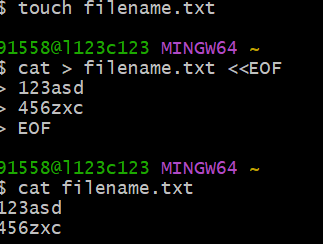
\includegraphics[width=0.5\linewidth]{touch.png}
  % 图片标题
  \captionof{figure}{创建写入读取文件}
  \label{fig:example}
\end{minipage}

8.创建目录与切换

\noindent
\begin{minipage}{\linewidth}
 \centering
  % 插入图片
  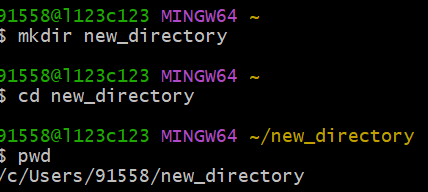
\includegraphics[width=0.5\linewidth]{mkdir.png}
  % 图片标题
  \captionof{figure}{创建与切换新目录}
  \label{fig:example}
\end{minipage}

9. 获取工作目录,并列出工作目录

\begin{minipage}{\linewidth}
    \centering
     % 插入图片
     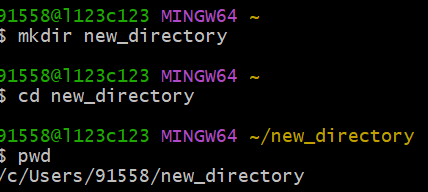
\includegraphics[width=0.5\linewidth]{mkdir.png}
     % 图片标题
     \captionof{figure}{获取目录并列出当前目录}
     \label{fig:example}
\end{minipage}


10.查看当前目录文件数目

\noindent
\begin{minipage}{\linewidth}
 \centering
  % 插入图片
  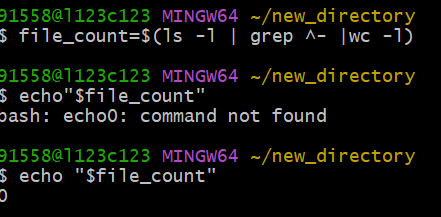
\includegraphics[width=0.5\linewidth]{file_count.png}
  % 图片标题
  \captionof{figure}{查看当前目录文件数目}
  \label{fig:example}
\end{minipage}



\subsection{Vim学习例子10个}
1.Vim文件的创立,
在终端中输入 vim example.txt


\noindent
\begin{minipage}{\linewidth}
  \centering
  % 插入图片
  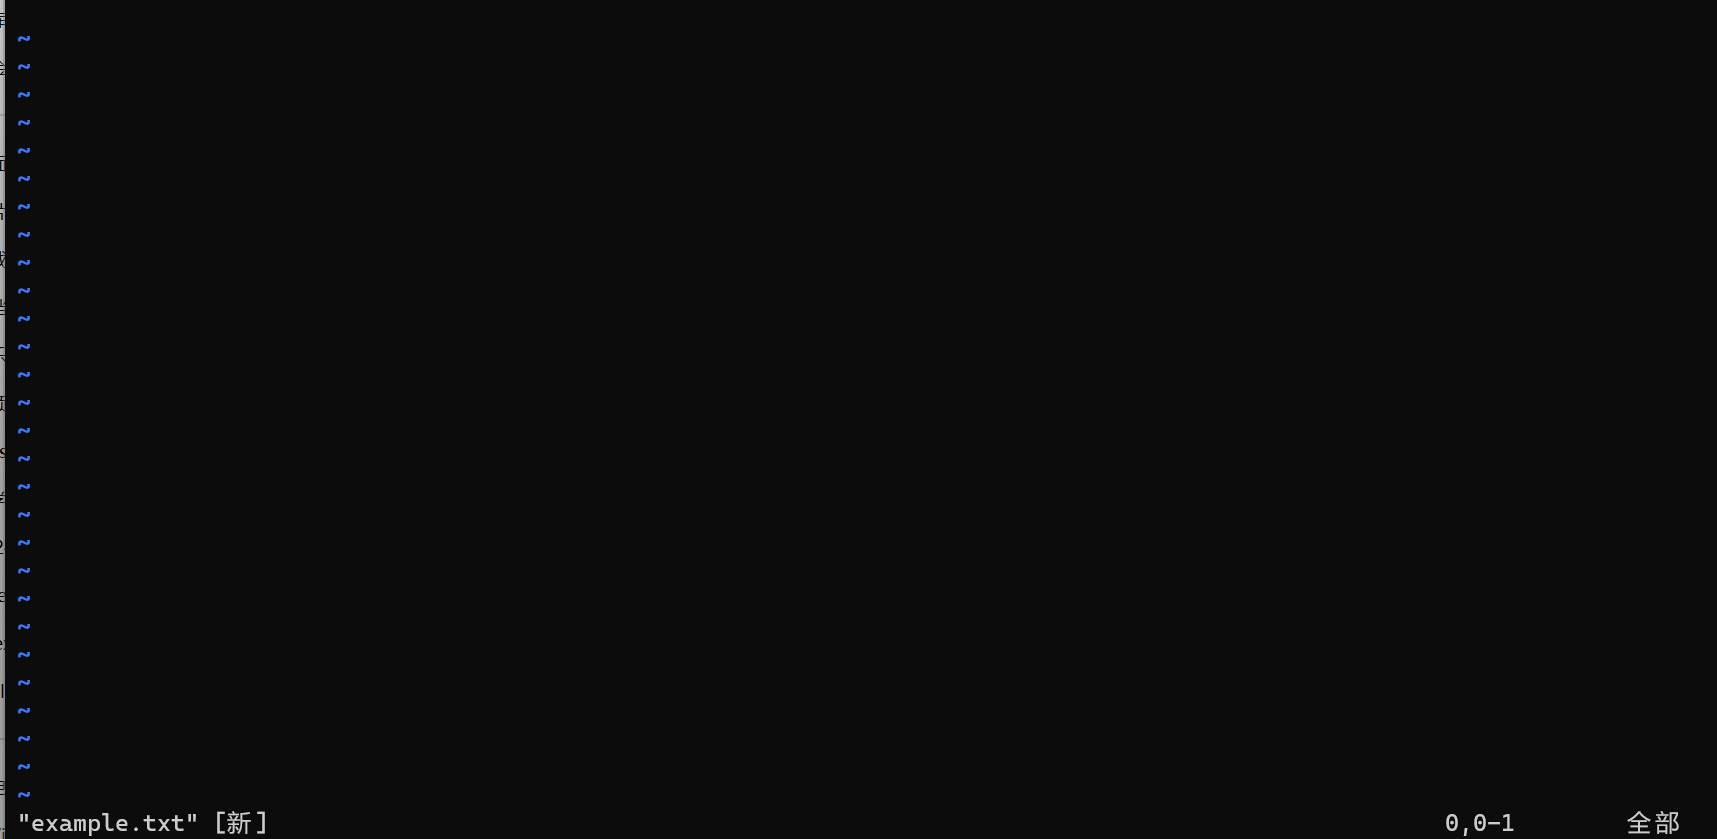
\includegraphics[width=0.5\linewidth]{vim1.png}
  % 图片标题
  \captionof{figure}{Vim文件的创立}
  \label{fig:example}
\end{minipage}

2. i键为插入,开始输入内容hello, vim!

\noindent
\begin{minipage}{\linewidth}
  \centering
  % 插入图片
  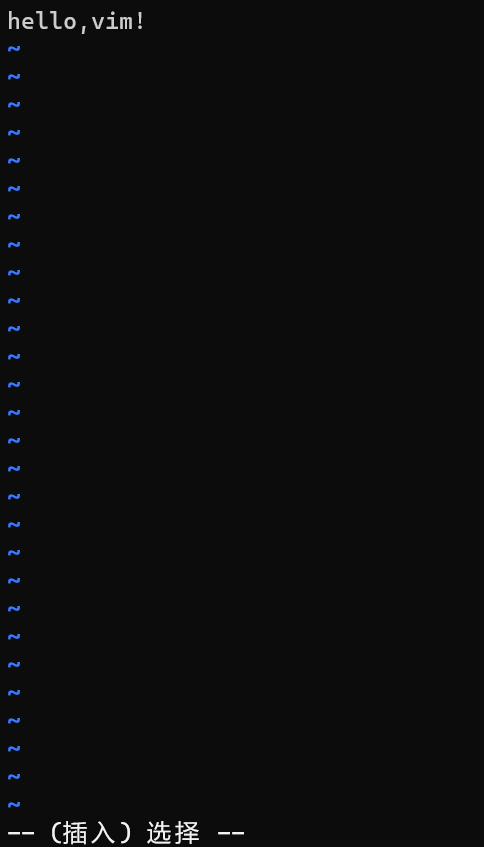
\includegraphics[width=0.5\linewidth]{vim2.png}
  % 图片标题
  \captionof{figure}{i插入内容}
  \label{fig:example}
\end{minipage}

3.编辑的退出与保存
\begin{verbatim}
   Esc是回到正常模式
   :w带编者保存
   :q代表退出
   如果不按w的话则文件为SWP文件,用于临时储存数据
\end{verbatim}

\noindent
\begin{minipage}{\linewidth}
 \centering
  % 插入图片
  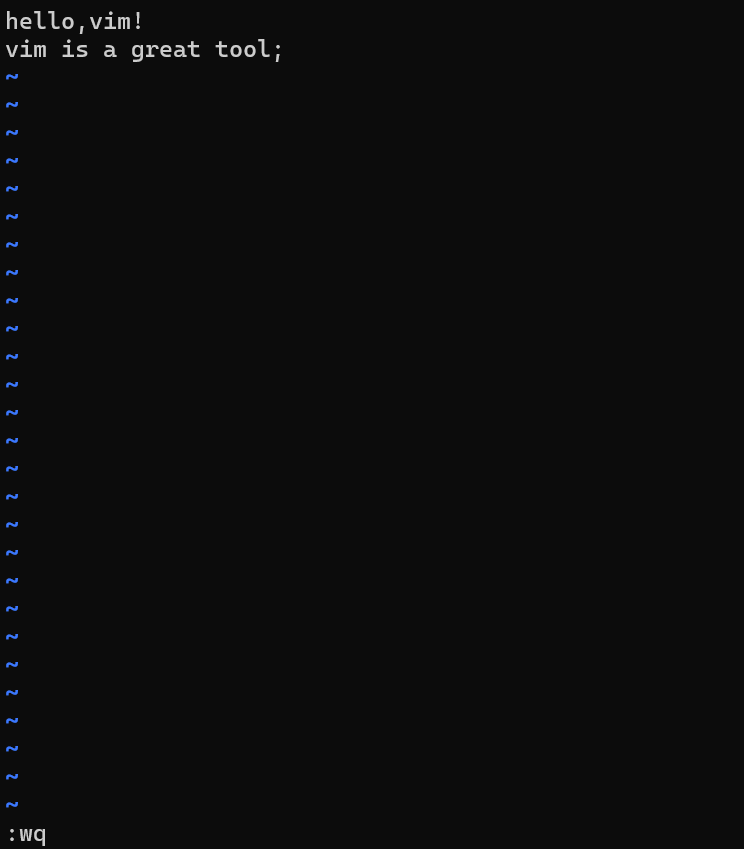
\includegraphics[width=0.5\linewidth]{vim3.png}
  % 图片标题
  \captionof{figure}{编辑的退出与保存}
  \label{fig:example}
\end{minipage}



4.dd表示删除当前行
\begin{verbatim}
   在vim is a greet tool前输入dd删除后的结果
\end{verbatim}


\noindent
\begin{minipage}{\linewidth}
 \centering
  % 插入图片
  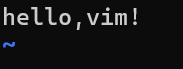
\includegraphics[width=0.5\linewidth]{vim4.png}
  % 图片标题
  \captionof{figure}{dd删除当前行后的结果}
  \label{fig:example}
\end{minipage}

5.dw:删除光标后的单词。

\noindent
\begin{minipage}{\linewidth}
 \centering
  % 插入图片
  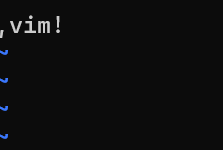
\includegraphics[width=0.5\linewidth]{vim5.png}
  % 图片标题
  \captionof{figure}{dw删除光标后的单词的结果}
  \label{fig:example}
\end{minipage}

6.x:删除光标下的字符。

\noindent
\begin{minipage}{\linewidth}
 \centering
  % 插入图片
  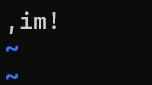
\includegraphics[width=0.5\linewidth]{vim6.png}
  % 图片标题
  \captionof{figure}{删除光标下的字符的结果}
  \label{fig:example}
\end{minipage}

7.r:替换光标下的单个字符。
R:进入替换模式,连续替换多个字符直到按下 Esc。


\noindent
\begin{minipage}{\linewidth}
 \centering
  % 插入图片
  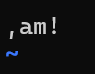
\includegraphics[width=0.5\linewidth]{vim7.png}
  % 图片标题
  \captionof{figure}{用r替换光标下的单个字符}
  \label{fig:example}
\end{minipage}

\noindent
\begin{minipage}{\linewidth}
 \centering
  % 插入图片
  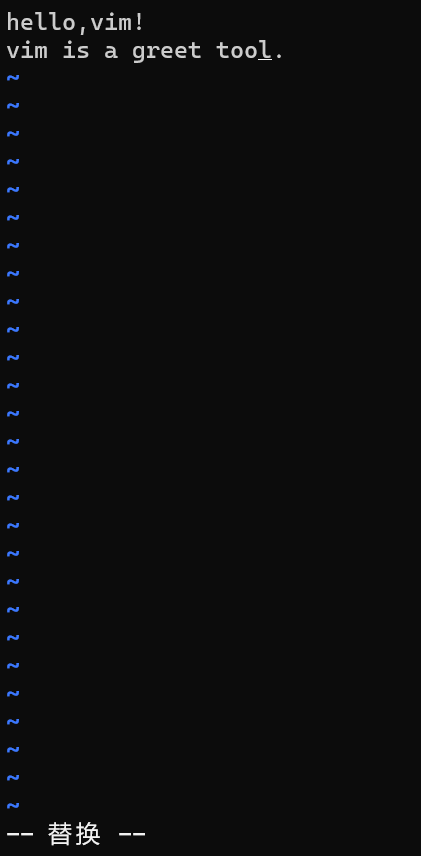
\includegraphics[width=0.5\linewidth]{vim8.png}
  % 图片标题
  \captionof{figure}{在R模式未改变前}
  \label{fig:example}
\end{minipage}

\noindent
\begin{minipage}{\linewidth}
 \centering
  % 插入图片
  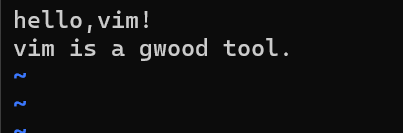
\includegraphics[width=0.5\linewidth]{vim9.png}
  % 图片标题
  \captionof{figure}{在R模式改变后}
  \label{fig:example}
\end{minipage}

8. 
u:撤销最后一次更改。

Ctrl + r:重做最后一次撤销,即反撤销。


\begin{minipage}{\linewidth}
    \centering
     % 插入图片
     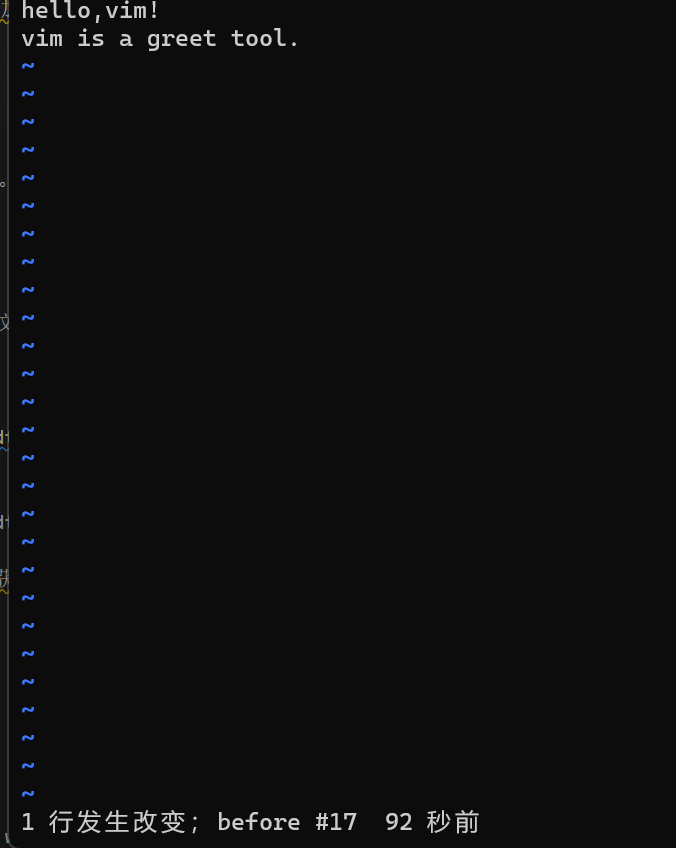
\includegraphics[width=0.5\linewidth]{vim10.png}
     % 图片标题
     \captionof{figure}{撤销}
     \label{fig:example}
\end{minipage}

\begin{minipage}{\linewidth}
  \centering
   % 插入图片
   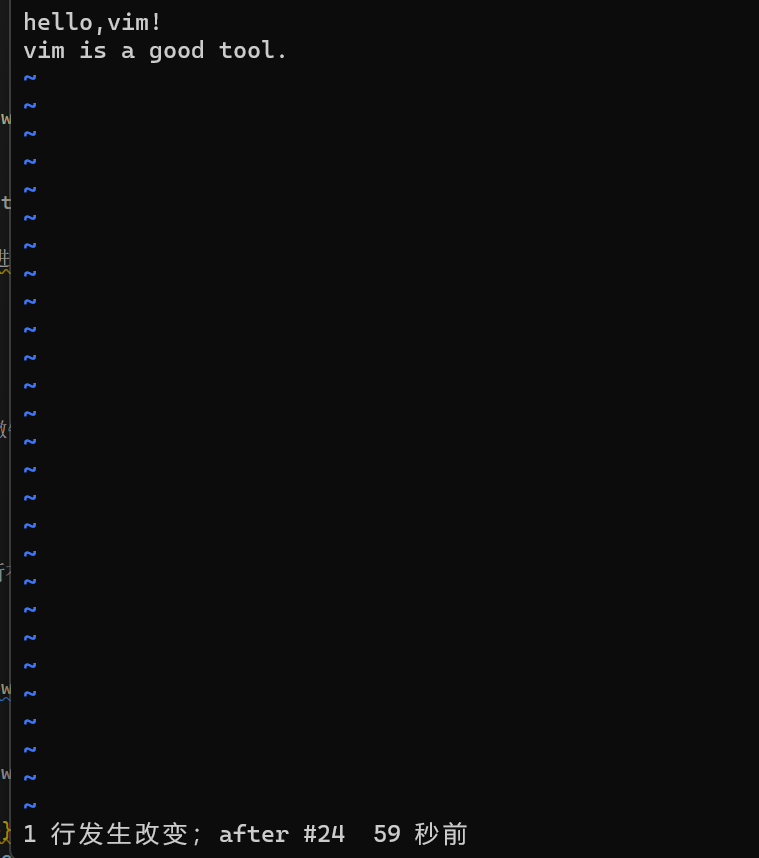
\includegraphics[width=0.5\linewidth]{vim11.png}
   % 图片标题
   \captionof{figure}{反撤销}
   \label{fig:example}
\end{minipage}


9.复制的学习:
单行:
将光标移动到要复制的行的任意位置。
输入 yy 来复制整行。

部分行:
将光标移动到要开始复制的位置。
进入可视化模式,可以按 v(用于字符模式)或 V(用于行模式)。
使用光标键hjkl选择要复制的文本。
一旦选择了文本,按 y 来复制选中的文本。

多个行:
将光标移动到要复制的第一行的任意位置。
输入 数字yy,其中 “数字” 是您想要复制的行数。
例如,3yy 会复制光标所在的当前行以及下面两行,总共三行。

\noindent
\begin{minipage}{\linewidth}
 \centering
  % 插入图片
  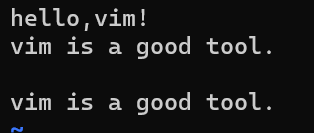
\includegraphics[width=0.5\linewidth]{vim12.png}
  % 图片标题
  \captionof{figure}{复制一行后的结果}
  \label{fig:example}
\end{minipage}

\noindent
\begin{minipage}{\linewidth}
 \centering
  % 插入图片
  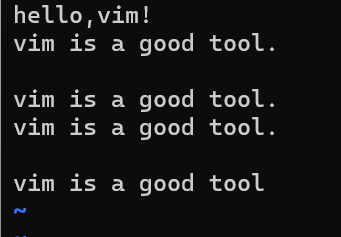
\includegraphics[width=0.5\linewidth]{vim13.png}
  % 图片标题
  \captionof{figure}{选择性复制后的结果}
  \label{fig:example}
\end{minipage}


10.
p:在光标后粘贴。
P:在光标前粘贴。
下面是粘贴后的结果

\noindent
\begin{minipage}{\linewidth}
 \centering
  % 插入图片
  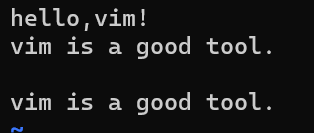
\includegraphics[width=0.5\linewidth]{vim12.png}
  % 图片标题
  \captionof{figure}{粘贴后的结果}
  \label{fig:example}
\end{minipage}




\section{解题感悟}
Shell是一种强大的自动化工具。通过编写脚本,日常繁琐的任务会变得简单高效,

Vim的也是一种更高效的工具。虽然学习过程有艰辛,但是新的习惯一旦形成,它将带来巨大的收益。

github路径
您可以在此查看项目的源代码: 

\url{https://github.com/L-c-hang/homework_two/}


\end{document}
